\documentclass[11pt]{article}
%\usepackage{amssymb}
%\usepackage{epsfig}
\usepackage{latexsym}
\usepackage{graphicx}
\usepackage{cite}
\usepackage{epsfig}
\usepackage{amsmath}
\usepackage{subfigure}
\usepackage{float}
\usepackage[usenames,dvipsnames]{color}

\newcommand{\commentaar}[1]{\colorbox{Yellow}{\begin{minipage}{0.5\linewidth}#1\end{minipage}}}
%\documentclass[10pt]{article}
%\usepackage{oz2e}
%\usepackage{a4}
%\usepackage[all]{xy}
\frenchspacing
\setlength{\parskip}{1ex plus0.5ex minus0.5ex}
\setlength{\parindent}{0cm}
%\textheight     9.2in
%\textwidth      6in


\begin{document}
\bibliographystyle{alpha}
\title{VJoint tree structuring\\
 DRAFT VERSION }
\author{Herwin van Welbergen \\
} \maketitle

\newpage
%\tableofcontents
\newpage

%\input{macros}

\section{Introduction}
This document describes the animation/rendering structure that supports splitting the rendering and animating processes into two seperate threads. To allow this (and in the future possibly to allow multiple remote visualisations of the animation process running on a server), we seperate the rendering and animation VJoint scene graphs (see Figure \ref{figuresg}). The local transform of the nodes under animation root is coupled to the render scene at its initialization. This coupling is many-to-one: one or more animation VJoints can steer a single render node. For example: a render node containing a deformable mesh for a humanoid is steered by a tree of animation VJoints representing the skeleton that steers the mesh. \commentaar{Klopt dit, of zitten ze nog wel als VJoints in de render tree?} The animation tree is coupled to the render tree using the VJoint rotation/translation buffers: setting the rotation or translation of a animation tree VJoint directly sets the rotation in the corresponding render node. If animation and rendering occurs in different threads, access to the animation tree should be synchronized. This prevents the render thread reading partial information from the animation scene while it is still being updated by the animation thread. Typically the animation processes uses of copies of parts of the animation tree locally in time consuming animation processes and then uses a synchronized copy action to copy the resulting VJoint transformations to the animation scene. The render thread uses a synchronized action to calculate the global render node transformations from rotations in the animation tree (see also Figure \ref{threads}).


\begin{figure}
\includegraphics[width=13cm]{typical_scenegraph-crop}
\caption{\label{figuresg}Typical scenegraph layout}
\end{figure}

\begin{figure}
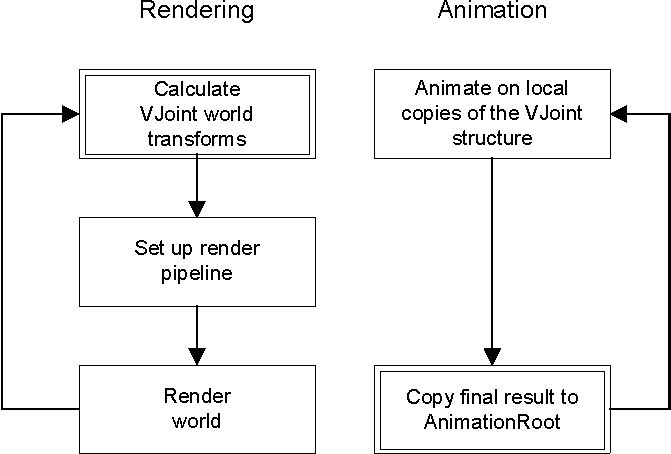
\includegraphics{threads-crop}
\caption{\label{threads}Animation and rendering loops running in different threads. The processes with double lines are synchronized to each other.}
\end{figure}

\end{document}
